\documentclass[12pt, oneside]{report}\usepackage[]{graphicx}\usepackage[]{color}
% maxwidth is the original width if it is less than linewidth
% otherwise use linewidth (to make sure the graphics do not exceed the margin)
\makeatletter
\def\maxwidth{ %
  \ifdim\Gin@nat@width>\linewidth
    \linewidth
  \else
    \Gin@nat@width
  \fi
}
\makeatother

\usepackage{Sweavel}


\usepackage[margin=0.85in]{geometry}
\linespread{1}
\usepackage{xcolor}
\usepackage[colorlinks=false, linkbordercolor=white, citebordercolor=white, 
    filebordercolor=white, urlbordercolor=white]{hyperref}
    
\usepackage{graphicx}
\usepackage[utf8]{inputenc}
\usepackage[english]{babel}
\usepackage[T1]{fontenc}

\usepackage{fancyhdr}
\pagestyle{fancy}
\renewcommand{\headrulewidth}{0.4pt}
\fancyhead{}
  \fancyhead[L]{Statistics for Computer Science -- assignment 1} %%% change to your course name and change the number accordingly
\fancyhead[R]{Kanitha Chim} %%% change to your first name and surname
\fancyfoot{}
\fancyfoot[C]{\thepage}

\usepackage{titlesec}
\titlespacing{\chapter}{0pt}{*4}{*2.5}

\titleformat{\chapter}{\normalfont\huge\bf}{\thechapter}{20pt}{\huge\bf}


% Setting up of environment
\usepackage{listings}
\definecolor{dgray}{gray}{0.35} % colour of comments
\definecolor{lgray}{gray}{0.95} % background colour of R-code
\definecolor{llgray}{gray}{0.98} % background colour of R-outputs

\lstdefinestyle{Rstyle}{ % settings of R-code style
language=R, % setting language R
basicstyle=\ttfamily\small, % font and size of R-code
backgroundcolor=\color{lgray}, % background colour of R-code
commentstyle=\ttfamily\small\itshape\color{dgray}, % colour of R comments
showstringspaces=false, % forbidding the highlighting of spaces
numbers=left, % numbering on the left
numberstyle=\ttfamily\small, % font and size of numbering
stepnumber=1, % numbering with step 1
firstnumber=last, % cumulative numbering of rows in consecutive Chunks
breaklines=T} % automatic line breaks of code at the end of a line

\lstdefinestyle{Routstyle}{ %  settings of R-output style
language=R, % setting language R
basicstyle=\ttfamily\small, % font and size of R-output
backgroundcolor=\color{llgray}, % background colour of R-code
showstringspaces=false, % forbidding the highlighting of spaces
numbers=right, % numbering on the right
numberstyle=\ttfamily\small, % font and size of numbering
firstnumber=last, % cumulative numbering of rows in consecutive Chunks
breaklines=T} % automatic line breaks of code at the end of a line

\begin{document}



\begin{titlepage}
    \begin{center}
        \vspace*{1cm}
        
        \Huge
          \textbf{Statistics for Computer Science} %%% change to your course name
        
        \vspace{0.5cm}
        \LARGE
        Assignment 1 %%% change the number accordingly
        
        \vspace{1.5cm}
        
        \textbf{Kanitha Chim} %%% change to your first name and surname
   		  \vspace{1.5cm}
        
        \textbf{501453} %%% change to your UCO
       
        \vfill
        
        Field of Study Software System and Service Management %%% change to your field of study
        
        \vspace{0.8cm}
          \Large
        Faculty of Informatics\\
        Masaryk University\\
        \vspace{0.5cm}
       \today
        
    \end{center}
\end{titlepage}

\addtocontents{toc}{~\hfill\textbf{Page}\par}

\section*{Exercise 1}
\noindent 1. Create your own R-functions for calculating estimates of the following characteristics: sample
mean, sample five number summary, sample skewness, sample kurtosis, sample variance, sample
standard deviation, sample range, sample decile range, sample 0.1-trimmed average and sample
0.1-trimmed variance. Use Cramér’s estimates for skewness and kurtosis. Do not use in-
built functions min(), max(), mean(), quantile(), var(), sd(), range() or functions from external
libraries.

\subsection*{Implementation in R}

\begin{Schunk}
\begin{Sinput}
#function to calculate minimum
cal_minimum <- function(x){
  x <- sort(x)
  min_val <- x[1]
  return(min_val)
}

#function to calculate maximum
cal_maximum <- function(x){
  x <- sort(x)
  max_val <- tail(x,1)
  return(max_val)
}

#median, first quartile, thrid quartile, quartile_type should be, one, two(median), or three
cal_quartile <- function(x, quartile_type){
  x <- sort(x)
  result <- 0
  
  if(quartile_type == 'two'){
    if(length(x) %% 2 == 0){
      return((x[length(x)/2] + x[length(x+1)/2])/2)
    }else{
      return(x[length(x+1)/2])
    }
  }else if(quartile_type == 'one'){
    position <- (length(x) + 1)/4
    if (floor(position) == ceiling(position)){
      return(x[position])
    }else{
      return((x[floor(position)] + x[ceiling(position)])/2)
    }
  }else if(quartile_type == 'three'){
    position <- (3*(length(x) + 1))/4
    if (floor(position) == ceiling(position)){
      return(x[position])
    }else{
      return((x[floor(position)] + x[ceiling(position)])/2)
    }
  }
}

#Sample mean
cal_mean <- function(x){
  result <- sum(x) / length(x)
  return(result)
}

#Sample five number summary
cal_five_num_summary <- function(x){
  min <- cal_minimum(x)
  q1 <- cal_quartile(x, 'one')
  q2 <- cal_quartile(x, 'two')
  q3 <- cal_quartile(x, 'three')
  max <- cal_maximum(x)
  return(c(min, q1, q2, q3, max))
  # return(list(min, q1, q2, q3, max))
}

#Sample Skewness
cal_coef_skew <- function(x){
  s <- sqrt(cal_sample_variance(x))
  mean <- cal_mean(x)
  total <- 0
  for(i in x){
    total = total + (i - mean)^3
  }
  
  return(total/(s^3 * length(x)))
  
}

#Sample Kurtosis
cal_coef_kurt <- function(x){
  s <- sqrt(cal_sample_variance(x))
  mean <- cal_mean(x)
  total <- 0
  for(i in x){
    total = total + (i - mean)^4
  }
  total = total/(s^4 * length(x))
  return(total -3)
}

#Sample Variance
cal_sample_variance <- function(x){
  mean <- cal_mean(x)
  n_minus_one <- length(x) - 1
  total <- 0
  for(i in x){
    total = total + (i - mean)^2
  }
  return(total/n_minus_one)
}

#Sample Standard Deviation
cal_sd <- function(x){
  sample_variance <- cal_sample_variance(x)
  return(sqrt(sample_variance))
}

#Sample Range
cal_sample_range <- function(x){
  return(cal_maximum(x) - cal_minimum(x))
}

#Sample Decile Range
cal_sample_decile_range <- function(x){
  x_0.9 <- 90/100 * (length(x) +1)
  x_0.1 <- 10/100 * (length(x) +1)
  
  if (floor(x_0.9) == ceiling(x_0.9)){
    x_0.9 = x_0.9
  }else{
    x_0.9 = (x[floor(x_0.9)] + x[ceiling(x_0.9)])/2
  }
  
  if (floor(x_0.1) == ceiling(x_0.1)){
    x_0.1 = x_0.1
  }else{
    x_0.1 = (x[floor(x_0.1)] + x[ceiling(x_0.1)])/2
  }
  return(x_0.9 - x_0.1)
}

#Sample 0.1 trimmed average
cal_sample_0.1_trimmed_average <- function(x){
  g <- abs(0.1 * length(x))
  n <- length(x)
  total <- 0
  for(i in seq(g+1, n-g, 1)){
    total <- total + x[i]
  }
  return(total/(n - 2*g))
}

#Sample 0.1 trimmed variance
cal_sample_0.1_trimmed_variance <- function(x){
   g <- abs(0.1 * length(x))
   n <- length(x)
   x_gt <- cal_sample_0.1_trimmed_average(x)
   total <- 0
   for(i in seq(g+1, n-g, 1)){
     total <- total + (x[i] - x_gt)^2
   }
   return(total/(n - 2*g - 1))
}

library(xtable)
\end{Sinput}
\end{Schunk}

\noindent 2. Separately for each population calculate sample size and these characteristics of maximum cranial breadth. Print them in a table with values rounded to 4 decimal places.

\subsection*{Implementation in R}
\begin{Schunk}
\begin{Sinput}
setwd('/home/jane/Documents/SSME (Service Development Management)/Term2/MV013-Statistics for Computer Science/Assignment1')
Howell <- read.csv('Howell.csv')
Howell.Male <- Howell[Howell$Sex == 'M', ]
Howell.Male.Australi <- Howell.Male[(Howell.Male$Population == 'AUSTRALI'), ]
Howell.Male.Peru <- Howell.Male[(Howell.Male$Population == 'PERU'), ]

#Working on population of 'AUSTRALI'
Australi.sample_size <- length(Howell.Male.Australi$XCB)
Australi.sample_mean <- cal_mean(Howell.Male.Australi$XCB)
Australi.sample_five_num_summary <- cal_five_num_summary(Howell.Male.Australi$XCB)
Australi.sample_skewness <- cal_coef_skew(Howell.Male.Australi$XCB)
Australi.sample_kurtosis <- cal_coef_kurt(Howell.Male.Australi$XCB)
Australi.sample_variance <- cal_sample_variance(Howell.Male.Australi$XCB)
Australi.sample_sd <- cal_sd(Howell.Male.Australi$XCB)
Australi.sample_range <- cal_sample_range(Howell.Male.Australi$XCB)
Australi.sample_decile_range <- cal_sample_decile_range(Howell.Male.Australi$XCB)
Australi.sample_0.1_trimmed_average <- cal_sample_0.1_trimmed_average(Howell.Male.Australi$XCB)
Australi.sample_0.1_trimmed_variance <- cal_sample_0.1_trimmed_variance(Howell.Male.Australi$XCB)

#Working on population of 'PERU'
Peru.sample_size <- length(Howell.Male.Peru$XCB)
Peru.sample_mean <- cal_mean(Howell.Male.Peru$XCB)
Peru.sample_five_num_summary <- cal_five_num_summary(Howell.Male.Peru$XCB)
Peru.sample_skewness <- cal_coef_skew(Howell.Male.Peru$XCB)
Peru.sample_kurtosis <- cal_coef_kurt(Howell.Male.Peru$XCB)
Peru.sample_variance <- cal_sample_variance(Howell.Male.Peru$XCB)
Peru.sample_sd <- cal_sd(Howell.Male.Peru$XCB)
Peru.sample_range <- cal_sample_range(Howell.Male.Peru$XCB)
Peru.sample_decile_range <- cal_sample_decile_range(Howell.Male.Peru$XCB)
Peru.sample_0.1_trimmed_average <- cal_sample_0.1_trimmed_average(Howell.Male.Peru$XCB)
Peru.sample_0.1_trimmed_variance <- cal_sample_0.1_trimmed_variance(Howell.Male.Peru$XCB)

Peru <- data.frame(Peru=c(Peru.sample_size, Peru.sample_mean, Peru.sample_five_num_summary, Peru.sample_skewness,
                        Peru.sample_kurtosis, Peru.sample_variance, Peru.sample_sd, Peru.sample_range,
                        Peru.sample_decile_range, Peru.sample_0.1_trimmed_average, Peru.sample_0.1_trimmed_variance),
                  row.names = c('Size', 'Mean', 'Minimum', 'Q1', 'Q2', 'Q3', 'Maximum', 'Skewness', 'Kurtosis', 'Variance',
                        'Standard Deviation', 'Range', 'Decile Range', 'Sampe 0.1 trimmed average', 'Sample 0.1 trimmed variance'))

Australi <- data.frame(Australi=c(Australi.sample_size, Australi.sample_mean, Australi.sample_five_num_summary, Australi.sample_skewness, 
                        Australi.sample_kurtosis, Australi.sample_variance, Australi.sample_sd, Australi.sample_range,
                        Australi.sample_decile_range, Australi.sample_0.1_trimmed_average, Australi.sample_0.1_trimmed_variance),
                       row.names = c('Size', 'Mean', 'Minimum', 'Q1', 'Q2', 'Q3', 'Maximum', 'Skewness', 'Kurtosis', 'Variance',
                        'Standard Deviation', 'Range', 'Decile Range', 'Sampe 0.1 trimmed average', 'Sample 0.1 trimmed variance'))

library(xtable)
\end{Sinput}
\end{Schunk}

\noindent 3. Create boxplots of maximum cranial breadth of each population side by side in one figure. Set the width of boxes to be proportional to sample sizes, add notches and arithmetic averages for both groups.

\subsection*{Implementation in R}
\begin{Schunk}
\begin{Sinput}
max.len = max(length(Howell.Male.Australi$XCB), length(Howell.Male.Peru$XCB))
x=c(Howell.Male.Australi$XCB, rep(NA, max.len - length(Howell.Male.Australi$XCB)))
y=c(Howell.Male.Peru$XCB, rep(NA, max.len - length(Howell.Male.Peru$XCB)))
Populations <- c('Australi', 'Peru')
values <- c(x, y)
df <- data.frame(Populations, values)

library(ggplot2)
boxplot <- ggplot(df, aes(x=Populations, y=values, fill=Populations)) +
          geom_boxplot(notch = TRUE, width=(55/110)) +
          scale_fill_manual(values=c("lightblue", "lightgreen")) +
          ylab('Maximum cranial breadth') +
          xlab('Populations') +
          annotate("text", x=1, y=Australi.sample_mean, label= round(Australi.sample_mean, 4)) +
          annotate("text", x=2, y=Peru.sample_mean, label= round(Peru.sample_mean, 4)) +
          ggtitle('Boxplot of maximum cranial breadth') +
          theme(plot.title = element_text(hjust = 0.5))
\end{Sinput}
\end{Schunk}

\noindent 4. Separately for each population create histogram of maximum cranial breadth. Make sure that the histograms can be easily compared (without using back-to-back histogram).
\subsection*{Implementation in R}
\begin{Schunk}
\begin{Sinput}
Australi.hist <- ggplot(data=data.frame(Australi=c(Howell.Male.Australi$XCB)), aes(x=Howell.Male.Australi$XCB)) + 
                geom_histogram(color="darkblue", fill="lightblue", binwidth = 1) + 
                xlab('Maximum cranial breadth of Australi') +
                ylab('Frequecy') +
                scale_x_continuous(breaks = seq(124, 144, 2), lim = c(122, 146)) + 
                geom_text(stat = 'count', aes(label =..count.., vjust = -0.5))

Peru.hist <- ggplot(data=data.frame(Peru=c(Howell.Male.Peru$XCB)), aes(x=Howell.Male.Peru$XCB)) + 
            geom_histogram(color="darkgreen", fill="lightgreen", binwidth = 1) + 
            xlab('Maximum cranial breadth of Peru') + 
            ylab('Frequency') +
            scale_x_continuous(breaks = seq(129, 149, 2), lim = c(128, 150)) + 
            geom_text(stat = 'count', aes(label =..count.., vjust = -0.5))
\end{Sinput}
\end{Schunk}


\noindent 5. Create normal qq-plot of maximum cranial breadth for each population.
\subsection*{Implementation in R}
\begin{Schunk}
\begin{Sinput}
Australi.qq <- ggplot(data=data.frame(Australi=c(Howell.Male.Australi$XCB))) + 
                aes(sample= Australi) + 
                geom_qq(distribution = qnorm) + 
                geom_qq_line(line.p = c(0.25, 0.75), col = "lightblue") + 
                ylab('Maximum cranial breadth for Australi') + 
                ggtitle('QQ-Plot of maximum cranial breadth of Australi') + 
                theme(plot.title = element_text(hjust = 0.5))

Peru.qq <- ggplot(data=data.frame(Peru=c(Howell.Male.Peru$XCB))) + 
            aes(sample= Peru) + 
            geom_qq(distribution = qnorm) + 
            geom_qq_line(line.p = c(0.25, 0.75), col = "lightgreen") + 
            ylab('Maximum cranial breadth for Peru') + 
            ggtitle('QQ-Plot of maximum cranial breadth of Peru') + 
            theme(plot.title = element_text(hjust = 0.5))
\end{Sinput}
\end{Schunk}

\noindent 6. Interpret your results and graphics.
\noindent Text. Results in table or graphic form. Commentaries and interpretation of the results.\\

\begin{center}
Characteristics of maximum cranial breadth \\
\end{center}

% latex table generated in R 3.6.3 by xtable 1.8-4 package
% Fri Apr 10 23:32:39 2020
\begin{tabular}{|l|l|}
  \hline
 & Australi \\ 
  \hline
Size &  52.0000 \\ 
  Mean & 131.9423 \\ 
  Minimum & 124.0000 \\ 
  Q1 & 128.0000 \\ 
  Q2 & 131.0000 \\ 
  Q3 & 134.0000 \\ 
  Maximum & 144.0000 \\ 
  Skewness &   0.6436 \\ 
  Kurtosis &  -0.3390 \\ 
  Variance &  26.0554 \\ 
  Standard Deviation &   5.1045 \\ 
  Range &  20.0000 \\ 
  Decile Range &  15.0000 \\ 
  Sampe 0.1 trimmed average & 129.4712 \\ 
  Sample 0.1 trimmed variance &  26.3226 \\ 
   \hline
\end{tabular}
% latex table generated in R 3.6.3 by xtable 1.8-4 package
% Fri Apr 10 23:32:39 2020
\begin{tabular}{|l|l|}
  \hline
 & Peru \\ 
  \hline
Size &  55.0000 \\ 
  Mean & 137.9455 \\ 
  Minimum & 129.0000 \\ 
  Q1 & 135.0000 \\ 
  Q2 & 138.0000 \\ 
  Q3 & 141.0000 \\ 
  Maximum & 149.0000 \\ 
  Skewness &  -0.0037 \\ 
  Kurtosis &   0.0616 \\ 
  Variance &  15.8673 \\ 
  Standard Deviation &   3.9834 \\ 
  Range &  20.0000 \\ 
  Decile Range &  -4.0000 \\ 
  Sampe 0.1 trimmed average & 138.1364 \\ 
  Sample 0.1 trimmed variance &  15.1438 \\ 
   \hline
\end{tabular}


\begin{Schunk}


{\centering 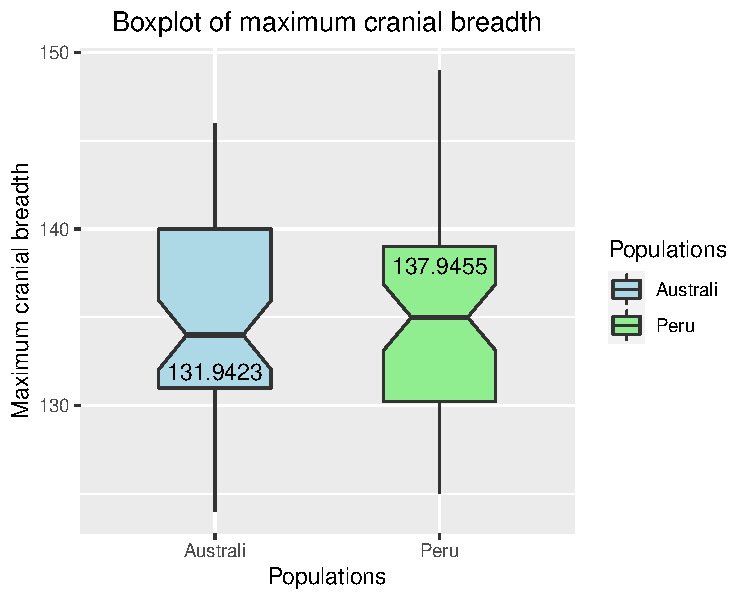
\includegraphics[width=\maxwidth]{figure/unnamed-chunk-7-1} 

}

\end{Schunk}

\begin{center}
Histograms represent maximum cranial breadth of each population \\
\end{center}

\begin{Schunk}

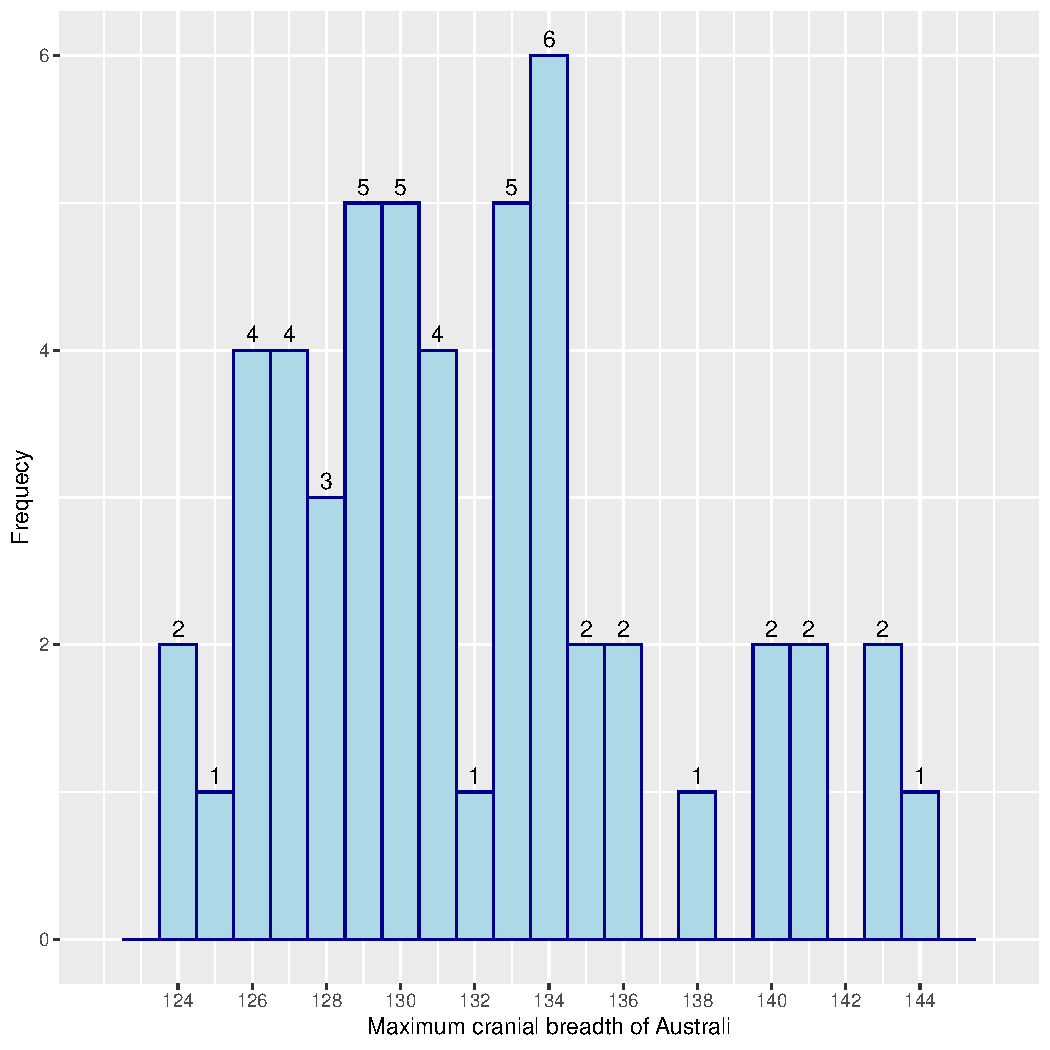
\includegraphics[width=8cm,height=8cm]{figure/unnamed-chunk-8-1} 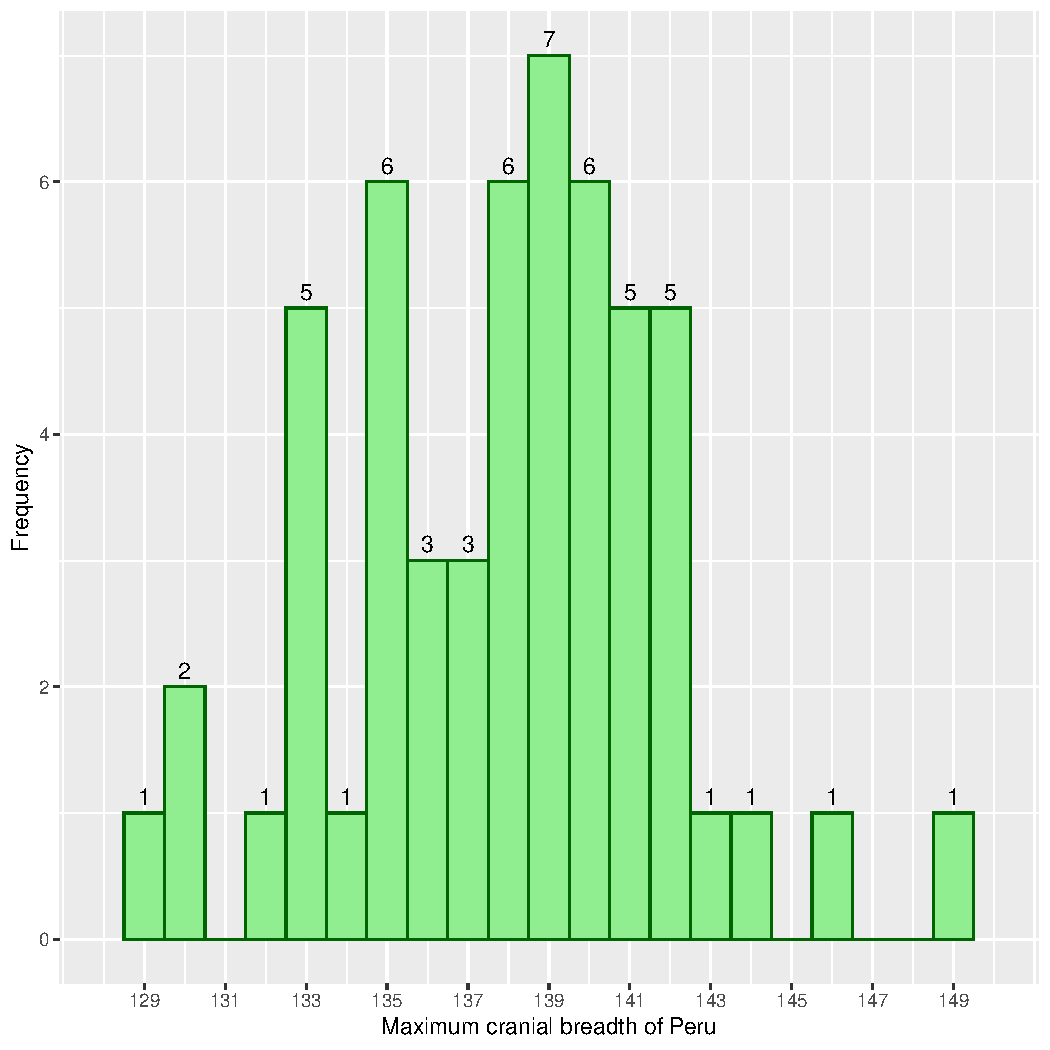
\includegraphics[width=8cm,height=8cm]{figure/unnamed-chunk-8-2} \end{Schunk}
\newpage
\begin{center}
QQ-plot represent maximum cranial breadth of each population \\
\end{center}

\begin{Schunk}

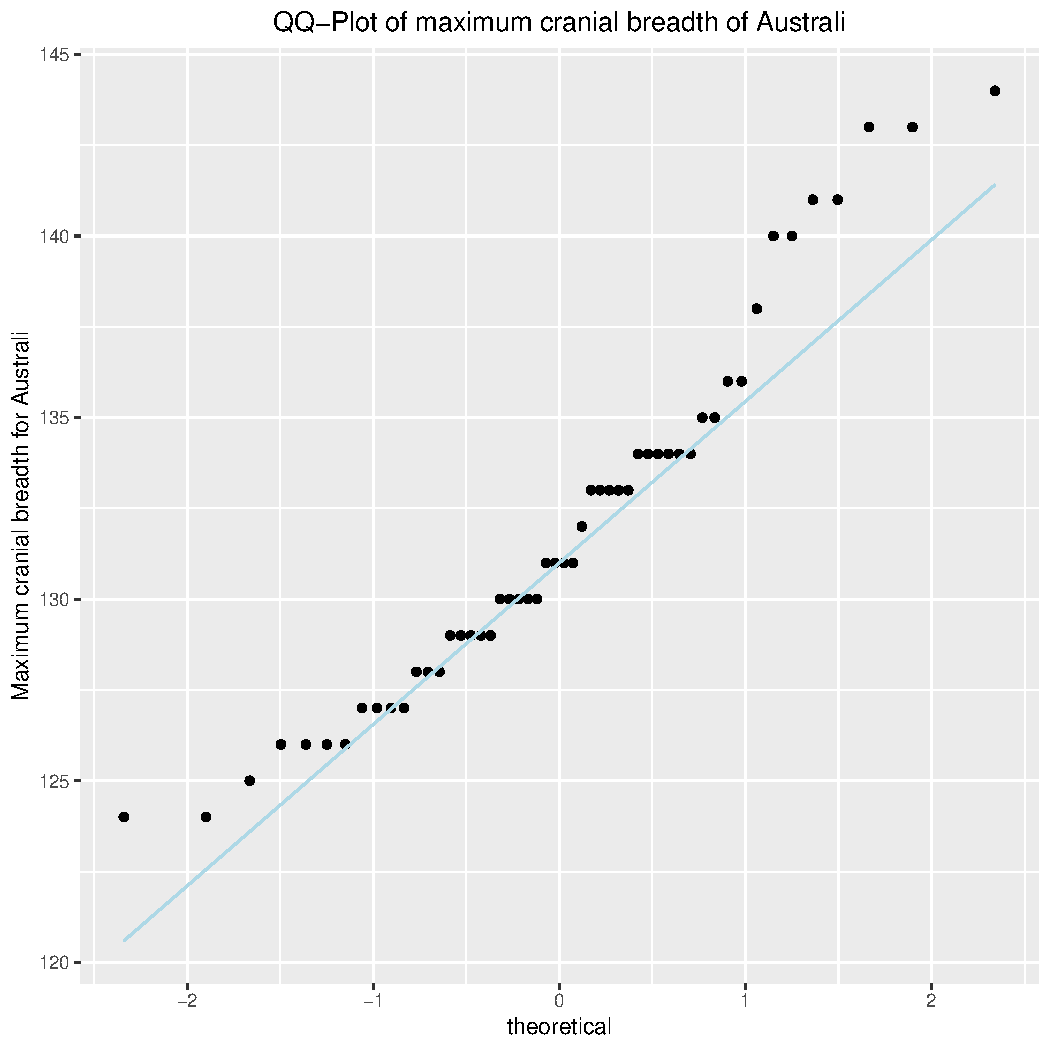
\includegraphics[width=8cm,height=8cm]{figure/unnamed-chunk-9-1} 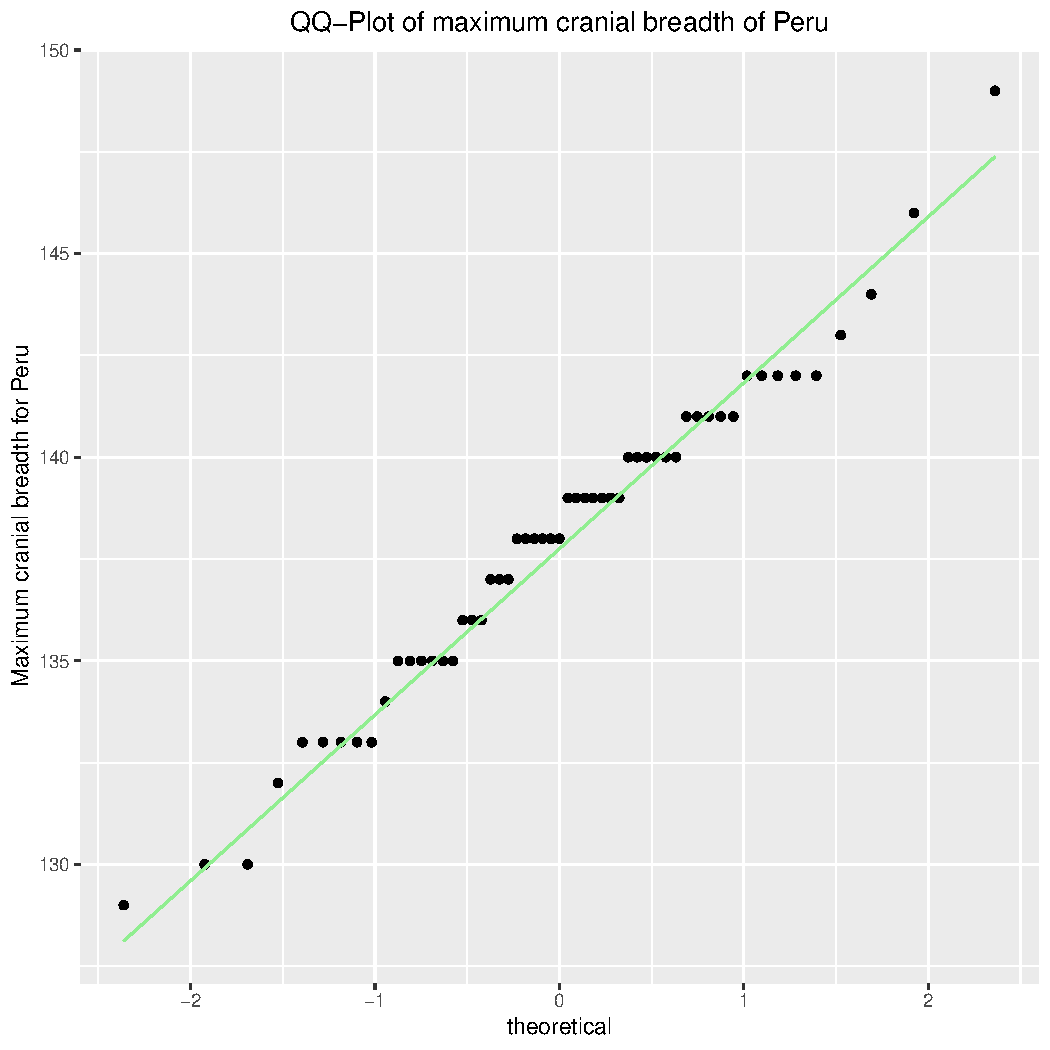
\includegraphics[width=8cm,height=8cm]{figure/unnamed-chunk-9-2} \end{Schunk}

\section*{Exercise 2}
\noindent 1. Calculate the number of men and women in Spain for each year and print them in a table together with the total population.

\subsection*{Implementation in R}
\begin{Schunk}
\begin{Sinput}
setwd('/home/jane/Documents/SSME (Service Development Management)/Term2/MV013-Statistics for Computer Science/Assignment1')
Spanish.province <- read.csv('area_spanish_provinces.csv')
Spanish.population <- read.csv('population-spain-1998-2018.csv', sep=";")

population.2018 <- sum(Spanish.population$males.2018, Spanish.population$females.2018)
population.2013 <- sum(Spanish.population$males.2013, Spanish.population$females.2013)
population.2008 <- sum(Spanish.population$males.2008, Spanish.population$females.2008)
population.2003 <- sum(Spanish.population$males.2003, Spanish.population$females.2003)
population.1998 <- sum(Spanish.population$males.1998, Spanish.population$females.1998)

total.population <- sum(colSums(Spanish.population[ ,-1]))

df <- data.frame(Male=c(sum(Spanish.population$males.1998), sum(Spanish.population$males.2003), 
                        sum(Spanish.population$males.2008), sum(Spanish.population$males.2013), 
                        sum(Spanish.population$males.2018), 0),
                 Female=c(sum(Spanish.population$females.1998), sum(Spanish.population$females.2003), 
                          sum(Spanish.population$females.2008), sum(Spanish.population$females.2013), 
                          sum(Spanish.population$females.2018), 0),
                 Total=c(population.1998, population.2003, population.2008, population.2013, population.2018, total.population))
row.names(df) <- c('1998', '2003', '2008', '2013', '2018', 'Total')
df[6,1] <- sum(df$Male)
df[6,2] <- sum(df$Female)
\end{Sinput}
\end{Schunk}

\noindent 2. Display barplot plot of total population of Spain in each of the years, with each bar divided
between men and women.

\subsection*{Implementation in R}
\begin{Schunk}
\begin{Sinput}
library(ggplot2)
year <- c(1998, 1998, 2003, 2003, 2008, 2008, 2013, 2013, 2018, 2018)
population <- c(sum(Spanish.population$males.1998), 
                sum(Spanish.population$females.1998), 
                sum(Spanish.population$males.2003), 
                sum(Spanish.population$females.2003), 
                sum(Spanish.population$males.2008), 
                sum(Spanish.population$females.2008), 
                sum(Spanish.population$males.2013), 
                sum(Spanish.population$females.2013), 
                sum(Spanish.population$males.2018), 
                sum(Spanish.population$females.2018))
gender <- c('Male', 'Female', 'Male', 'Female', 'Male', 'Female', 'Male', 'Female', 'Male', 'Female' )
df.population <- data.frame(year, population, gender)
population.barplot<-ggplot(data=df.population, aes(x=year, y=population, fill=gender )) +
  geom_col() +
  scale_fill_manual(values=c("lightpink", "lightblue")) +
  scale_x_continuous(breaks = seq(1998, 2018, 5)) + 
  # scale_y_continuous(breaks = sprintf("%.0fk", population/1000)) +
  geom_text(aes(label = sprintf("%.0fk", population/1000)), position = position_stack(0.5)) +
  theme(axis.text.y=element_text(angle = 45))
\end{Sinput}
\end{Schunk}

\noindent 3. Display barplot of relative proportions of men and women within each province in 2018
\subsection*{Implementation in R}
\begin{Schunk}
\begin{Sinput}
proportion.province <-c(as.vector(Spanish.population$province), as.vector(Spanish.population$province))
proportion.gender <- c(rep('Male', 52), rep('Female', 52))
proportion.province.gender <- c(proportion.male, proportion.female)
\end{Sinput}
\begin{Soutput}
Error in eval(expr, envir, enclos): object 'proportion.male' not found
\end{Soutput}
\begin{Sinput}
df.proportion <- data.frame(proportion.province, proportion.province.gender, proportion.gender)
\end{Sinput}
\begin{Soutput}
Error in data.frame(proportion.province, proportion.province.gender, proportion.gender): object 'proportion.province.gender' not found
\end{Soutput}
\begin{Sinput}
proportion.barplot <- ggplot(data=dffff, aes(x=proportion.province, y=proportion.province.gender, fill=proportion.gender)) + 
          geom_col() + 
          theme(axis.text.x=element_text(angle = 90, size=6), plot.title = element_text(vjust=0.5, hjust=1)) +
          scale_fill_manual(values=c("lightpink", "lightblue")) +
          scale_x_discrete(name= "Provinces") +
          scale_y_continuous(name= "Population proportion") + 
          ggtitle('Barplot of population proportion')
\end{Sinput}
\begin{Soutput}
Error in ggplot(data = dffff, aes(x = proportion.province, y = proportion.province.gender, : object 'dffff' not found
\end{Soutput}
\begin{Sinput}
proportion.barplot
\end{Sinput}
\begin{Soutput}
Error in eval(expr, envir, enclos): object 'proportion.barplot' not found
\end{Soutput}
\end{Schunk}


\noindent 5. Interpret your results and graphics.
% latex table generated in R 3.6.3 by xtable 1.8-4 package
% Fri Apr 10 23:32:41 2020
\begin{table}[ht]
\centering
\begingroup\large
\begin{tabular}{|l|l|l|l|}
  \hline
 & Male & Female & Total \\ 
  \hline
1998 & 19488465 & 20364186 & 39852651 \\ 
  2003 & 21034326 & 21682738 & 42717064 \\ 
  2008 & 22847737 & 23310085 & 46157822 \\ 
  2013 & 23196386 & 23933397 & 47129783 \\ 
  2018 & 22896602 & 23826378 & 46722980 \\ 
  Total & 109463516 & 113116784 & 222580300 \\ 
   \hline
\end{tabular}
\endgroup
\caption{Population of Spanish} 
\end{table}

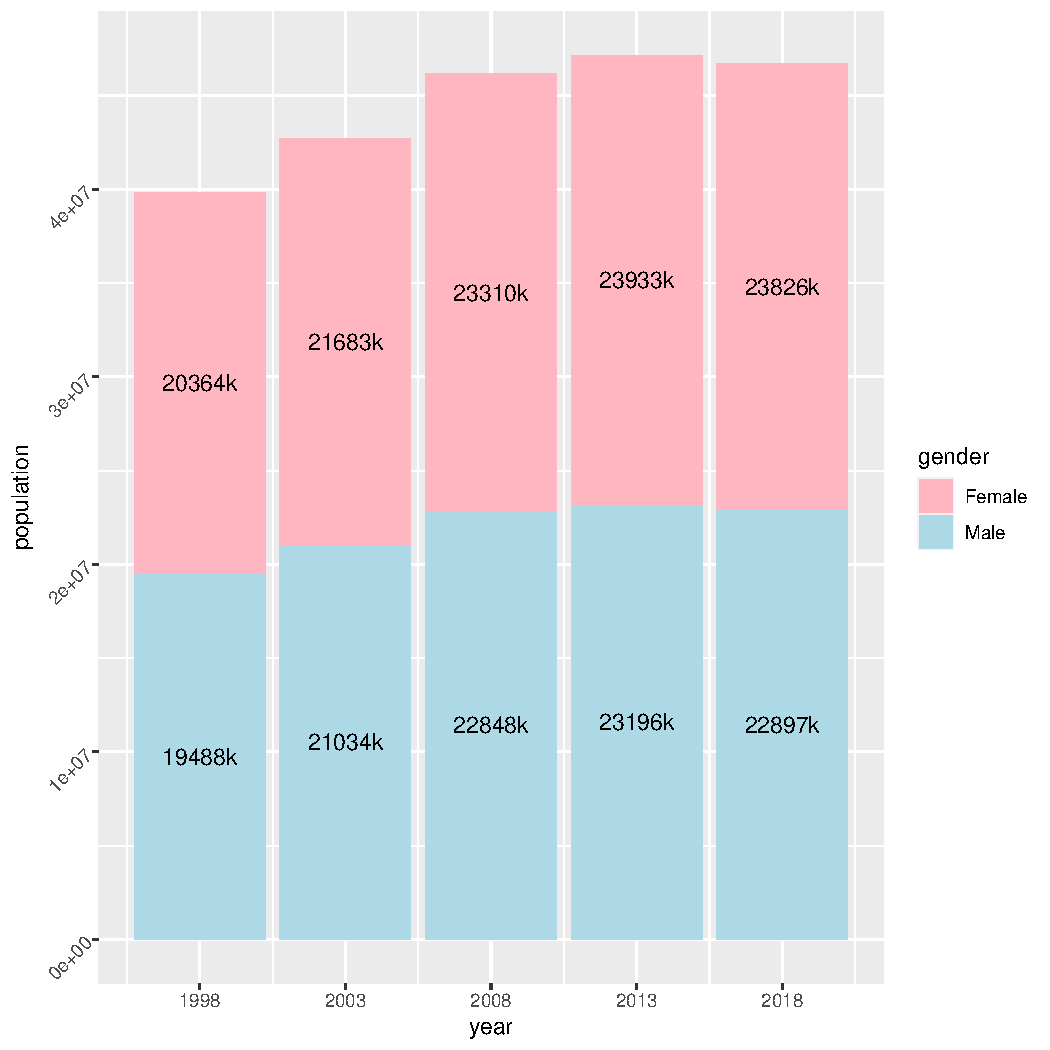
\includegraphics[width=\maxwidth]{figure/unnamed-chunk-13-1} 

\end{document}

